% Observer/Estimator
% Author: Dominik Haumann
\documentclass[tikz,convert={density=600,outext=.png}]{standalone}

\usepackage[utf8]{inputenc} % utf8 encoding
\usepackage[english]{babel}
\usepackage[T1]{fontenc} % use T1 fonts
\usepackage{amsmath} % nice math symbols
     

\usepackage{tikz}
\usetikzlibrary{shapes,positioning,calc}

\begin{document}

	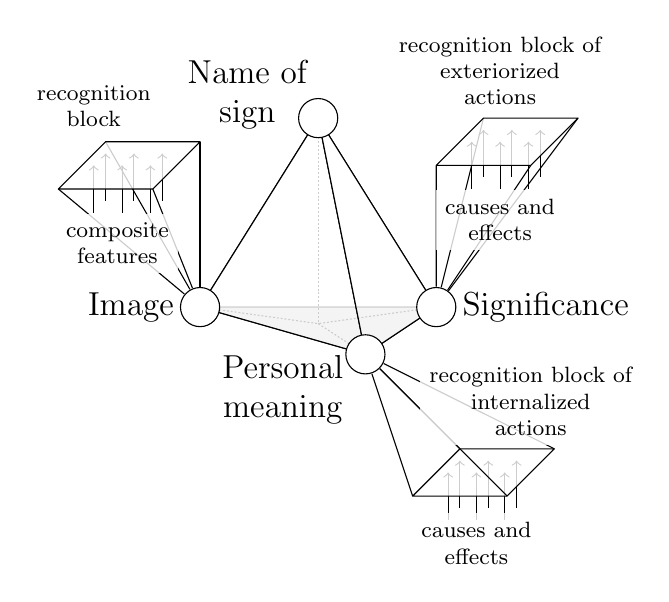
\begin{tikzpicture}[join=round,scale=3.0,node distance = -0.05]
		%\draw[step=0.1,black,thin] (-1,0) grid (2,2);
	
		\tikzstyle{sign_comp}=[draw, circle,fill=white, scale=1.5];
		\tikzstyle{label_small}=[align=center,font=\footnotesize,fill=white,opacity=0.8,text opacity=1];
		\tikzstyle{coord_cine}=[dash pattern=on 0.7 off 0.7];
		
		\filldraw[fill=white] (0.0,0.2) -- (0.5,1.0) -- (1.0,0.2) -- cycle;
		\filldraw[fill=black!20] (0.0,0.2) -- (0.7,0.0) -- (1.0,0.2) -- cycle;

		\draw[coord_cine] (0.5,1.0) -- (0.5,0.13);
		\draw[coord_cine] (0.0,0.2) -- (0.5,0.13);
		\draw[coord_cine] (0.7,0.0) -- (0.5,0.13);
		\draw[coord_cine] (1.0,0.2) -- (0.5,0.13);

		\filldraw[fill=white,fill opacity=0.8] (0.0,0.2) -- (0.5,1.0) -- (0.7,0.0) -- cycle;
		\filldraw[fill=white,fill opacity=0.8] (0.7,0.0) -- (0.5,1.0) -- (1.0,0.2) -- cycle;
				
		\node[sign_comp] (s_p) at (0.0,0.2) {};
		\node[sign_comp] (s_m) at (1.0,0.2) {};
		\node[sign_comp] (s_n) at (0.5,1.0) {};
		\node[sign_comp] (s_a) at (0.7,0.0) {};
				
		\draw[thin] (-0.4,0.9) -- (s_p);
		\draw[thin] (0.0,0.9) -- (s_p);
		\draw[thin] (-0.2,0.7)  -- (s_p);
		\draw[thin] (-0.6,0.7) -- (s_p);
		\draw[thin,<-] (-0.45,0.8)--++(0.0,-0.2);
		\draw[thin,<-] (-0.33,0.8)--++(0.0,-0.2);
		\draw[thin,<-] (-0.21,0.8)--++(0.0,-0.2);
		\draw[thin,<-] (-0.40,0.85)--++(0.0,-0.2);
		\draw[thin,<-] (-0.28,0.85)--++(0.0,-0.2);
		\draw[thin,<-] (-0.16,0.85)--++(0.0,-0.2);
		\filldraw[fill=white,fill opacity=0.8] (-0.4,0.9) -- (0.0,0.9) -- (-0.2,0.7) -- (-0.6,0.7) -- cycle;
		\node[label_small] at ($(s_p)+(-0.35,0.27)$) {composite\\features};
		\node[label_small] at ($(s_p)+(-0.45,0.85)$) {recognition\\block};
		
		\draw[thin] (1.2,1.0) -- (s_m);
		\draw[thin] (1.6,1.0) -- (s_m);
		\draw[thin] (1.0,0.8)  -- (s_m);
		\draw[thin] (1.4,0.8) -- (s_m);
		\draw[thin,<-] (1.15,0.9)--++(0.0,-0.2);
		\draw[thin,<-] (1.27,0.9)--++(0.0,-0.2);
		\draw[thin,<-] (1.39,0.9)--++(0.0,-0.2);
		\draw[thin,<-] (1.20,0.95)--++(0.0,-0.2);
		\draw[thin,<-] (1.32,0.95)--++(0.0,-0.2);
		\draw[thin,<-] (1.44,0.95)--++(0.0,-0.2);
		\filldraw[fill=white,fill opacity=0.8] (1.2,1.0) -- (1.6,1.0) -- (1.4,0.8) -- (1.0,0.8) -- cycle;
		\node[align=center,font=\footnotesize,fill=white,opacity=0.8,text opacity=1] at ($(s_m)+(0.27,0.37)$) {causes and\\effects};
		\node[align=center,font=\footnotesize,fill=white,opacity=0.8,text opacity=1] at ($(s_m)+(0.27,1.0)$) {recognition block of\\exteriorized\\actions};
		
		\draw[thin,<-] (1.05,-0.5)--++(0.0,-0.2);
		\draw[thin,<-] (1.17,-0.5)--++(0.0,-0.2);
		\draw[thin,<-] (1.29,-0.5)--++(0.0,-0.2);
		\draw[thin,<-] (1.10,-0.45)--++(0.0,-0.2);
		\draw[thin,<-] (1.22,-0.45)--++(0.0,-0.2);
		\draw[thin,<-] (1.34,-0.45)--++(0.0,-0.2);
		\filldraw[fill=white,fill opacity=0.8] (1.1,-0.4) -- (1.5,-0.4) -- (1.3,-0.6) -- (0.9,-0.6) -- cycle;
		\draw[thin] (1.1,-0.4) -- (s_a);
		\draw[thin] (1.5,-0.4) -- (s_a);
		\draw[thin] (0.9,-0.6)  -- (s_a);
		\draw[thin] (1.3,-0.6) -- (s_a);
		\node[align=center,font=\footnotesize,fill=white,opacity=0.8,text opacity=1] at ($(s_a)+(0.47,-0.8)$) {causes and\\effects};
		\node[align=center,font=\footnotesize,fill=white,opacity=0.8,text opacity=1] at ($(s_a)+(0.7,-0.2)$) {recognition block of\\internalized\\actions};
				
		\node[left = of s_p, font=\large] {Image};
		\node[right = of s_m, font=\large]{Significance};
		\node[align=center, font=\large] at ($(s_n)+(-0.30,0.1)$) {Name of\\sign};
		\node[align=center, font=\large] at ($(s_a)+(-0.35,-0.15)$) {Personal\\meaning};		
	\end{tikzpicture}

\end{document}